\documentclass{beamer}

\usepackage[utf8]{inputenc}
\usepackage[spanish]{babel}
\usepackage{graphicx}

\xdefinecolor{rojito}{rgb}{1,0.3,0.3}
\xdefinecolor{oliva}{cmyk}{0.64,0,0.95,0.4}
\xdefinecolor{minaranja}{rgb}{0.94,0.48,0.2}

\usetheme{Madrid}
\usecolortheme[named=rojito]{structure}

\title[Computación Cuántica]{Introducción a la Computación Cuántica}
\author{Luis Aguirre \& Javier Pellejero}
\institute[UCM]{Universidad Complutense de Madrid\\ Facultad de Informática}

\newcommand{\filados}[2]{ \left. \begin{array}{c}	#1 \\	#2	 \end{array} \right. }
\newcommand{\filacuatro}[4]{ \left. \begin{array}{c}#1\\#2\\#3\\#4	\end{array} \right.}
\newcommand{\base}[1]{|#1\rangle}
\newcommand{\lbase}[1]{\langle#1|}
\newcommand{\dotproduct}[2]{\langle#1|#2\rangle}
\newcommand{\tensor}[2]{|#1\rangle\langle#2|}
\newcommand{\baseup}{\mid\uparrow\rangle}
\newcommand{\baseright}{\mid\rightarrow\rangle}
\newcommand{\baseupright}{\mid\nearrow\rangle}
\newcommand{\baseupleft}{\mid\nwarrow\rangle}
\newcommand{\complex}{\mathbb{C}}
\newcommand{\A}{\mathrm{a}}
\newcommand{\B}{\mathrm{b}}
\newcommand{\C}{\mathrm{c}}
\newcommand{\D}{\mathrm{d}}
\newcommand{\U}{\mathrm{u}}
\newcommand{\V}{\mathrm{v}}
\newcommand{\x}{\mathrm{x}}
\newcommand{\y}{\mathrm{y}}
\newcommand{\T}{\mathrm{T}}
\newcommand{\puertai}{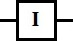
\includegraphics[scale=0.8]{imagenes/puertai}}
\newcommand{\puertax}{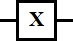
\includegraphics[scale=0.8]{imagenes/puertax}}
\newcommand{\puertay}{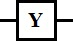
\includegraphics[scale=0.8]{imagenes/puertay}}
\newcommand{\puertaz}{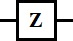
\includegraphics[scale=0.8]{imagenes/puertaz}}
\newcommand{\puertah}{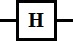
\includegraphics[scale=0.8]{imagenes/puertah}}
\newcommand{\puertacnot}{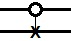
\includegraphics[scale=0.8]{imagenes/puertacnot}}

\begin{document}

\begin{frame}
	\titlepage
	\begin{center} Doble Grado en Matemáticas e Ingeniería Informática\end{center}
\end{frame}

\begin{frame}
\frametitle{Índice}
	\tableofcontents
\end{frame}

\section{Una primera aproximación mediante la polarización de fotones}

\begin{frame}
	\frametitle{Una aproximación mediante la polarización de fotones}
	Tenemos tres filtros de polarización de luz:
	\begin{itemize}
		\item \textbf{Filtro A:} de polarización horizontal $\rightarrow$.
		\item \textbf{Filtro B:} de polarización diagonal $\nearrow$.
		\item \textbf{Filtro C:} de polarización vertical $\uparrow$.
	\end{itemize}
\end{frame}

\begin{frame}
	\frametitle{Una aproximación mediante la polarización de fotones}
	Colocamos el \textbf{filtro A} tras una fuente de luz y vemos que los rayos han quedado polarizados horizontalmente con una intensidad de aproximadamente el 50 \%.
	\begin{center}
	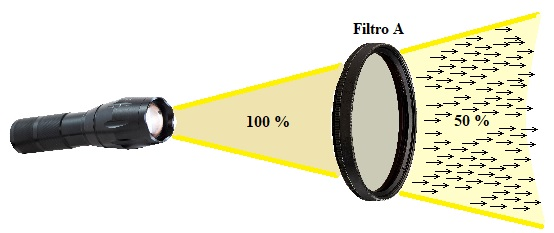
\includegraphics[scale=0.6]{imagenes/polarizacion1}\\
	Experimento 1.
	\end{center}
	Nótese que el filtro no sólo deja pasar a los rayos previamente polarizados horizontalmente. Debido a la aleatoriedad de la polarización de la fuente, que la mitad de los rayos tuviera dicha polarización exacta sería imposible.		
\end{frame}

\begin{frame}
	\frametitle{Una aproximación mediante la polarización de fotones}
	Ahora, tras el filtro A, colocamos el \textbf{filtro C}. Podemos observar que la luz que traspasa ambos filtros es nula.
	\begin{center}
	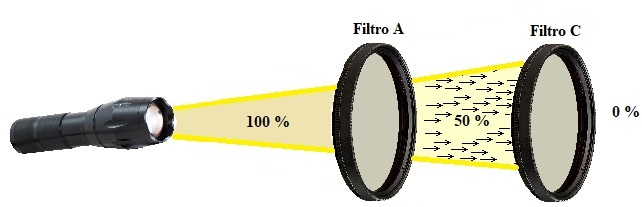
\includegraphics[scale=0.6]{imagenes/polarizacion2}\\
	Experimento 2.
	\end{center}		
\end{frame}

\begin{frame}
	\frametitle{Una aproximación mediante la polarización de fotones}
	Sin embargo, si ahora colocamos el \textbf{filtro B} entre ambas, sí que obtenemos luz 		tras traspasar todos los filtros, aunque sólo $\dfrac{1}{8}$ parte del original.
	\begin{center}
	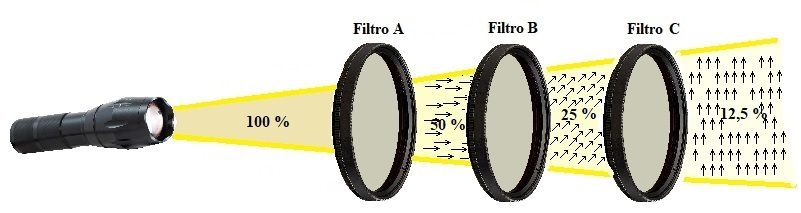
\includegraphics[scale=0.55]{imagenes/polarizacion3}\\
	Experimento 3.
	\end{center}
\end{frame}

\begin{frame}
	\frametitle{Una aproximación mediante la polarización de fotones}
	Conclusiones:
	\begin{itemize}
	\item Cada filtro realiza una ``medida'' que \textbf{cambia} la polarización de cada fotón. 
	\item Sean las bases $\baseup$ y $\baseright$, podemos denotar la polarización de un rayo cualquiera como $\base\psi =\ \A\baseup\ +\ \B\baseright$ con $\A,\B \in\complex$ y $|\A|^2+|\B|^2=1.$
	\item La medición de un rayo en esas bases obtendrá $\baseup$ con una probabilidad de $\A^2$ o $\baseright$ con una probabilidad de $\B^2$.
	\item Debido a la aleatoriedad inicial, aproximadamente un 50\% de los rayos serán reflejados (medición $\baseup$) y el resto los atravesará ($\baseright$).
	\item Tras la medición en el filtro A, todos los rayos tendrán el estado $\baseright = 0\baseup + 1\baseright$. Así, el filtro C refleja todos los rayos pues la probabilidad de medir $\baseup$ es cero.
	\end{itemize}
\end{frame}

\begin{frame}
	\frametitle{Una aproximación mediante la polarización de fotones}
	\begin{itemize}
	\item Colocando el filtro B cambiamos de base a $\{\baseupright, \baseupleft\}=$ $=\{\dfrac{1}{\sqrt{2}}(\baseup + \baseright), \dfrac{1}{\sqrt{2}}(\baseup - \baseright)\}$.
	\item Véase que $\baseright = \dfrac{1}{\sqrt{2}}(\baseupright - \baseupleft)$ y $\baseup = \dfrac{1}{\sqrt{2}}(\baseupright + \baseupleft)$.
	\item Así, la posibilidad de que al medir $\baseupright$ en el filtro B es de $\left(\dfrac{1}{\sqrt{2}}\right)^2=$ $=\dfrac{1}{2}$ y el estado de los rayos se proyectará en $\baseupright=\dfrac{1}{\sqrt{2}}(\baseup + \baseright)$.
	\item Por tanto, ahora sí podrán traspasar el filtro C, de nuevo con probabilidad $\dfrac{1}{2}$. Como cada filtro ha reflejado el 50\% de los rayos que le han llegado, sólo una octava parte ha traspasado los tres y tendrán estado $\baseup$.
	\end{itemize}
\end{frame}

\section{Estados cuánticos y notación}

\begin{frame}
	\frametitle{Estados cuánticos y notación}
	Sean $\base{\x}$ y $\base{\y}$ estados cuánticos.
	\begin{itemize}
	\item Denotamos $\lbase{\x}$ como el traspuesto de $\base{\x}$.
	\item Denotamos el producto escalar como $\lbase{\x}\base{\y}$ o simplemente $\dotproduct{\x}{\y}$.
	\item Denotamos el producto tensorial como $\tensor\x\y$.
	\end{itemize}
	
	\begin{block}{Ejemplo}
	Supongamos que trabajamos en la base $\{(1,0)^\T, (0,1)^\T\}$ que denotamos como $\{\base{0},\base{1}\}$.
	\begin{itemize}
	\item $\dotproduct 0 0 =1$ y $\dotproduct 0 1 =0$
	\item $\tensor 0 1 = \left({\begin{array}{c}   1\\0\\ \end{array} } \right)\left({\begin{array}{cc}   0 & 1\\ \end{array} } \right)=\left({\begin{array}{cc}   0 & 1\\ 0&0\\ \end{array} } \right)$
	\item Por tanto, $\tensor 0 1$ convierte $\base 1$ a $\base 0$ y $\base 0$ a $(0,0)^\T$.
	\end{itemize}
	\end{block}
\end{frame}


\begin{frame}
	\frametitle{Estados cuánticos y notación}
	\begin{block}{Definición}
	Definimos \textbf{bit cuántico} o \textbf{qubit} como un vector unitario complejo de dos dimensiones en una base ortonormal previamente fijada $\base 0$ y $\base 1$ que representa la  superposición de dos estados. Lo representamos como $\A\base0+\B\base1$ con $\A,\B\in\complex$ tal que $|\A|^2+|\B|^2=1$.
	\end{block}
	¿Qué pasa cuando tenemos múltiples qubit?
	\begin{itemize}
	\item En espacios clásicos, si V y W son espacios clásicos con bases $\{\mathrm{v}_1,\mathrm{v}_2\}$ y $\{\mathrm{w}_1,\mathrm{w}_2\}$ respectivamente, la ``unión'' de esos dos subespacios viene dada por el \textbf{producto cartesiano} de ambos que toma como base la unión de las anteriores $\{\mathrm{v}_1,\mathrm{v}_2,\mathrm{w}_1,\mathrm{w}_2\}$. Se cumple que la Dim(V$\times$W) = Dim(V) + Dim(W).
	\item Sin embargo, en espacios cuánticos, dicha ``unión'' viene dada por el \textbf{producto tensorial} que produce $\{\mathrm{v}_1\otimes\mathrm{w}_1,\mathrm{v}_1\otimes\mathrm{w}_2, \mathrm{v}_2\otimes\mathrm{w}_1,\mathrm{v}_2\otimes\mathrm{w}_2\}$.
	\end{itemize}
\end{frame}


\begin{frame}
	\frametitle{Estados cuánticos y notación}
	\begin{itemize}
	\item Así para dos qubits que tienen bases $\{\base0,\base1\}$ se genera $\{\base0\otimes\base0, \base0\otimes\base1, \base1\otimes\base0,\base1\otimes\base1\}$ o $\{\base{00},\base{01},\base{10},\base{11}\}$.
	\item Para 3 bits tendríamos $\{\base{000},\base{001},\base{010},\base{011},\base{100},\base{101},\base{110},\base{111}\}$.
	\item Se verifica así que Dim(V$\otimes$W) = Dim(V) $\times$ Dim(W).
	\item Sin embargo, no podemos alcanzar algunos estados en términos de sus componentes por separado. Por ejemplo $\base{00}+\base{11}$. Deberían existir $(\A_1\base0+\B_1\base1)\otimes(\A_2\base0+\B_2\base1)=$ $=\A_1\A_2\base{00}+\A_1\B_2\base{01}+\B_1\A_2\base{10}+\B_1\B_2\base{11}\neq\base{00}+\base{11}$ Puesto que $\A_1$ o $\B_2$ o ambos debe ser cero. 
	\end{itemize}
\end{frame}

\begin{frame}
	\frametitle{Estados cuánticos y notación}
	\begin{block}{Ejemplo. Medida en un sistema de 2 qubits.}
	Midamos el primer bit en la base $\{\base0,\base1\}$. Sea el estado $\A\base{00}+\B\base{01}+\C\base{10}+\D\base{11}$ con $|\A|^2+|\B|^2+|\C|^2+|\D|^2=1$. 
	\end{block}
	\begin{itemize}
	\item Lo reescribimos como $\base0(\A\base0+\B\base1)+\base1(\C\base0+\D\base1)=$ $=\U\base0\otimes(\frac{\A}{\U}\base0+\frac{\B}{\U}\base1) + \V\base0\otimes(\frac{\C}{\V}\base0+\frac{\D}{\V}\base1)$ con $\filados{\U=\sqrt{|\A|^2+|\B|^2}}{\V=\sqrt{|\C|^2+|\D|^2}}$.
	\item Nótese que $\frac{\A}{\U}\base0+\frac{\B}{\U}\base1$ y $\frac{\C}{\V}\base0+\frac{\D}{\V}\base1$ son vectores unitarios.
	\item Así la medida del primer qubit arrojará $\base0$ con probabilidad $\U^2$ y proyectará el estado $\base0\otimes(\frac{\A}{\U}\base0+\frac{\B}{\U}\base1)$.
	\item O arrojará $\base1$ con probabilidad $\V^2$ proyectando el estado $\base1\otimes(\frac{\C}{\U}\base0+\frac{\D}{\U}\base1)$.
	\end{itemize}
\end{frame}

\section{Paradoja EPR}

\begin{frame}
	\frametitle{Paradoja EPR}
\end{frame}

\section{Operaciones en sistemas cuánticos: Puertas cuánticas}

\begin{frame}
	\frametitle{Operaciones en sistemas cuánticos: Puertas cuánticas}
	\begin{block}{Definición}
	Definimos \textbf{puerta cuántica} como una transformación...	
	\end{block}
\end{frame}

\begin{frame}
	\frametitle{Operaciones en sistemas cuánticos: Puertas cuánticas}
	\textbf{Puertas simples (1 qubit):}
	\begin{itemize}
	\item Identidad I:$\filados{\base0\to\base0}{\base1\to\base1}$
	$\left({\begin{array}{cc}1&0\\0&1\end{array} } \right)$ \puertai
	
	\item Negación X:$\filados{\base0\to\base1}{\base1\to\base0}$
	$\left({\begin{array}{cc}0&1\\1&0\end{array} } \right)$ \puertax
	
	\item Combinación ZX Y:$\filados{\base0\to-\base{1}}{\base1\to\base0}$
	$\left({\begin{array}{cc}0&-1\\1&0\end{array} } \right)$ \puertay
	
	\item Cambio de fase Z:$\filados{\base0\to\base0}{\base1\to-\base1}$ 
	$\left({\begin{array}{cc}1&0\\0&-1\end{array} } \right)$ \puertaz
	
	\item Hadamard H:$\filados{\base0\to\dfrac{1}{\sqrt{2}}(\base0 + \base1)}{\base1\to\dfrac{1}{\sqrt{2}}(\base0 - \base1)}$ 
	$\left({\begin{array}{cc}1&0\\0&-1\end{array} } \right)$ \puertah
	\end{itemize}
\end{frame}

\begin{frame}
	\frametitle{Operaciones en sistemas cuánticos: Puertas cuánticas}
	\textbf{Otras puertas:}
	\begin{itemize}
	\item Cnot:$\filacuatro{\base{00}\to\base{00}}{\base{01}\to\base{01}}{\base{10}\to\base{11}}{\base{11}\to\base{10}}$
	$\left({\begin{array}{cccc}1&0&0&0\\0&1&0&0\\0&0&0&1\\0&0&1&0\end{array} } \right)$ \puertacnot
		\begin{itemize}
		\item El primer bit actúa como bit de control, cambiando el valor del segundo si el del primero es 1.
		\item No puede ser compuesta como producto tensorial de transformaciones de dos bits individuales.
		\end{itemize}
	
	
	\end{itemize}
\end{frame}

\end{document}
